\chapter{Nuclear structure and deformations}
In this chapter, a concise introduction to nuclear physics is provided, as a way to understand the essential physical properties of the system under study.
First, in section \ref{sec:models}, we will review the main empirical facts about nuclides, such as particle density distribuion and binding energies and the  simple phenomenological models historically employed to describe them. Moving on to more advanced topics, that are able to complete the general description of nuclear structure, which are nuclear pairing in section \ref{sec:pairing_intro} and nuclear deformations in section \ref{sec:deformations}.
\\Lastly, in section \ref{sec:fission}, we will overview the nuclear fission process, by deriving a simple model to describe it and discussing the importance of exotic deformations to accurately describe it.
\label{chap:intro}
\section{Nuclear structure models}
\label{sec:models}
The study of low energy hadron physics, has always been a challenging task. This is due to the known fact that the strong force, which is responsible for the attraction between the nucleons in a nuclei, is not perturbative at low energies, as opposed to the atomic case for the Coulomb interaction.
\subsection{Phenomenology of the NN interaction}
It is possible to obtain a good insight on the nuclear structure, by using empirical data obtained experimentally on the more macroscopic properties of nuclei, such as the binding energy and the particle density.
\subsubsection{Binding energies}
Let us start by the omnipresent physical quantity that is the binding energy of a nucleus. We can define it as the mass defect of the nucleus with respect to the constituents -- protons and neutrons -- isolated from eachother. If Z is the number of protons, N the number of neutrons, and $A=N+Z$ the nuclear mass, then the binding energy $E_B$ is given by
\begin{equation}
    \label{eq:binding_energy}
    E_B = (Zm_p + Nm_n - M)c^2
\end{equation}
where $m_p$ is the proton mass, $m_n$ the neutron mass, and $M$ the nucleus mass.
\\In figure \ref{fig:BE}, the binding energy per nucleon $E_B/A$ of nuclei as a function of $A$ is plotted. As shown in the figure, the binding energy per nucleon rapidly saturates and stalls around $7$ MeV just after $A=4$, this striking behaviour is due to nucleons interacting only with near neighbours, since the strong force is a short-range interaction, otherwise, the trend would follow a behaviour of $A(A-1)$ as in the Coulomb case.
\begin{figure}[h]
    \centering
    \includegraphics[width=0.6\textwidth]{Images/BE.png}
    \caption{Binding energy per nucleon as a function of $A$. Due to the short range of the strong force, this value saturates around $7$ MeV, with a steady, dim decrease after $^{56}$Fe.}
    \label{fig:BE}
\end{figure}
\subsubsection{Nuclear density}
An important aspect of nuclear phenomenology which can be easily obtained through electron scattering experiments \cite{Hofstadter1956} is the nuclear density. It can be very well represented by a Fermi-like distribution, which reads
\begin{equation}
    \label{eq:phen_density}
    \rho(r)=\frac{\rho_0}{1+e^{\frac{r-R_0}{a}}},
\end{equation}
where $R_0$ is the nuclear radius, which can be parametrized as $R_0\approx 1.2A^{1/3}$, and $a$ is the diffusivity, whose value determines how sharp the density drops from its saturation value $\approx \rho_0$ to $\approx 0$. The saturation density $\rho_0$ is generally universal for all nuclei, amounting to $\approx 0.16$ fm$^{-3}$.
\subsection{Nuclear models}
The formal description of nuclear structure has been proven to be a difficult task over the years. Due to the extremely rich phenomenology of nuclei and the challenges brought by the strong force, as we shall see, many models and further approximations to give a satisfactory description of all nuclides have been proposed.
\subsection{Liquid drop model}
One, if not the first successful model, is the liquid drop model. It is based on the assumption that the nucleus behaves as a liquid droplet, where forces among consituents tend to saturate. This hypothesis, formulated by G. Gamow, culminated in the formalization of the semi-empirical mass formula (SEMF) by N. Bohr and C. F. von Weizsäcker in 1935 \cite{Weizsacker1935}, which reads
\begin{equation}
    \label{eq:semf}
    E_B=a_V A - a_S A^{2/3} - a_C \frac{Z(Z-1)}{A^{1/3}} - a_A \frac{(N-Z)^2}{A} + \delta_P
\end{equation}
where $E_B$ is the binding energy of the nucleus. Each term has a different physical meaning:
\begin{itemize}
    \item $a_V A$ is the volume energy of the nucleus, given by the approximately constant binding energy per nucleon, which makes the total energy roughly proportional to $A$;
    \item $a_S A^{2/3}$ is the surface energy, a correction to the volume energy due to outer nuclei -- on the surface -- interacting with fewer nucleons than those in the inner bulk;
    \item $a_C Z(Z-1)/A^{1/3}$ is the approximation to the Coulomb energy repulsion of the nucleus, assuming the protons are uniformely distributed;
    \item $a_A (N-Z)^2/A$ is the asymmetry energy, which is due to the Pauli exclusion principle, since protons and neutrons occupy their respective states, a high imbalance of one species or the other implies loosely bound nucleons, thus a higher energy contribution of those states; and
    \item $\delta_P$ refers to the pairing energy of the nucleus, whose parametrization and physical significance will be later discussed in section \ref{sec:pairing_intro}.
\end{itemize}
\begin{figure}[h]
    \centering
    \includegraphics[width=1.0\textwidth]{Images/Liquid_drop_model.pdf}
    \caption{Visual representation of the liquid drop model from \cite{ldmimg}}
    \label{fig:liquid_drop_model}
\end{figure}
The SEMF can be fitted on current data to get a good estimate of binding energies \cite{Benzaid2020}, but it still lacks the ability of describing many aspects of nuclear structure, mainly, the nuclear shell structure, which can account for magic numbers and nuclear deformations.
\subsection{Shell corrections}
Describing the nucleus through a shell model would account for the quantum mechanical nature of the system, unfortunately, unlike the `atomic' case, we don't have a source of the field to which nucleons are sucjected to, since it's generated by the nucleons themselves; nonetheless, the formulation of an empirical potential which reproduces experimental data has been proven to be successful in providing useful corrections to the liquid drop model.
\\The so called Woods-Saxon potential is an empirical field used for modelling the average field to which an independent nucleon would feel in a nucleus. It can take different parametrizations depending on the data that one wants to reproduce. It is formulated as to follow the shape of the nuclear density \eqref{eq:phen_density}, and it reads
\begin{equation}
    \label{eq:sphWS}
    U(\bm r) = -\frac{U_0(A, N)}{1+e^\frac{r - R}{a}}
\end{equation}
where $U_0$ is the potential depth
\begin{equation}
    U_0(A, N) = U_0\bigg(1\pm \kappa \frac{2N -A }A\bigg),
\end{equation}
the $+$ and $-$ signs refer to protons and neutrons respectively. $R$ refers to the radius of the nuclear surface, generally parametrized as 
\begin{equation}
    R=r_0 A^{1/3}
\end{equation}
and $a$ is the surface diffuseness, as in the density expression \eqref{eq:phen_density}.
\paragraph{Spin-orbit coupling} 
The success of the shell model is mainly due to the possibility of accounting for spin-orbit coupling, which is included through a term that reads
\begin{equation}
    U_{\text{LS}}(\bm r )=U_0^{\text{LS}}\bigg(\frac{r_0}{\hbar}\bigg)^2 \frac 1 r \dv{}{r}\bigg (\frac{1}{1+e^{\frac{r-R}{a}}}\bigg).
\end{equation}
\paragraph{Coulomb interaction}
In the spherical case, the coulomb interaction can be taken as the energy potential produced by a sphere of charge $Z$ and radius $R$, which reads
\begin{equation}
    U_{\text{C}}(r) = Ze^2
    \begin{cases}
        \frac{3-(r/R)^2}{2R} & r \le R, \\
        \frac 1 r & r > R.
    \end{cases}
\end{equation}
The complete Hamiltonian then reads
\begin{equation}
    \hat H = \hat T + U + U_{\text{LS}}+U_C,
\end{equation}
where $U_C$ is present only when solving for the proton shells. The solution to the eigenvalue problem $\hat H \psi = E\psi$ is of the form
\begin{equation}
   \psi_{nljm_j} = \frac{u_{nl}(r)}{r}[Y_{l}(\hat {\bm r})\otimes \chi_{1/2}]_{jm_j} 
\end{equation}
where $Y_{nl}(\hat {\bm r})$ is the spherical harmonic function of degree $l$ and order $m$, the $\hat r$ is used to denote dependence on the azimuthal and polar angles of $\bm r$ and $\otimes$ takes the meaning of the angular momentum coupling and $u_{nl}(r)$ satisfies the reduced Schr\"odinger equation
\begin{equation}
    \label{eq:red}
    \bigg(-\frac {\hbar^2}{2m}\dv[2]{r}+\frac{\hbar l(l+1)}{2mr^2}+U(r)\bigg)\psi_{nl} = E\psi_{nl}.
\end{equation}
The effect of the spin-orbit coupling $U_{\text{LS}}$ and the Coulomb repulsion $U_C$ can be accounted for by using first order perturbation theory.
\subsubsection{Harmonic oscillator}
A small digression on the harmonic oscillator is in order. The solution of the spherical potential 
\begin{equation}
U_{\text{HO}} (\bm r ) = \frac 1 2 m\omega^2 r^ 2,
\end{equation}
produces the spherical harmonic oscillator basis, which is very similar to the basis one would get solving for the Woods-Saxon potential, provided that $\omega$ is taken as $41/A^{1/3}$ MeV. As a matter of fact, the harmonic oscillator basis is often used to perform calculations in nuclear physics. We will see in section \ref{sec:minimization} that a harmonic oscillator basis is used as starting guess for the numerical solution of a Woods-Saxon potential.
\subsubsection{Shell structure}
A graphical representation of the shells for a harmonic oscillator is shown in figure \ref{fig:shell_model}, where the contribution of the spin-orbit coupling is also accounted for; unlike the atomic case, shells whose total angular momentum is higher are lowered in energy, viceversa for lower total angular momentum.  
\begin{figure}[h]
    \centering
    \includegraphics[width=0.5\textwidth]{Images/ShellModel.png}
    \caption{Graphical representation of a harmonic oscillator shells, together with the spin-orbit coupling. Shells whose total angular momentum is higher are lowered in energy, viceversa for lower total angular momentum.}
    \label{fig:shell_model}
\end{figure}



\section{Nuclear pairing}
\label{sec:pairing_intro}
In the semi-empirical mass formula \eqref{eq:semf}, the $\delta_p$ term is parametrised as 
\begin{equation}
    \delta_p = \begin{cases}
        +\delta_0 & \text{ if N and Z are even}, \\
        0 & \text{ if A is odd}, \\
        -\delta_0 & \text{ if N and Z are odd},
    \end{cases}
\end{equation}
hence having an even number of neutrons and/or protons increases the binding energy of the nucleus. A common choice for $\delta_0$ is
\begin{equation*}
\delta_0 = 12 A^{1/2}\text{ MeV}.
\end{equation*}
This is a phenomena closely related to superconductivity, as nucleons of the same type form pairs that lie in higher energy states. An experimental evidence of this fact is knwon as odd-even staggering, where the separation energy
\begin{equation}
    S_n = E_B(A, Z) - E_B(A-1, Z),
\end{equation}
is higher for even $A$, an increase that corresponds to the energy necessary to break a pair. We will see in section \ref{sec:pairing_hf} the two main methods to account for pairing at a microsopic level.



\section{Nuclear deformations}
\label{sec:deformations}
If we were to observe the ratio between the first and second excited states energies of even-even nuclei, respectively $E(2^+)$ and $E(4^+)$, we would find that for nuclei where both $N$ and $Z$ are far from magic numbers, the ratio could be well approximated as 
\begin{equation}
    \label{eq:ratio}
    \frac{E(4^+)}{E(2^+)} \approx 3.33.
    \end{equation}
The ratio \eqref{eq:ratio} can be explained by the collective rotation of the nucleus, when rotational symmetry is broken. Denoting by $J$ the total angular momentum of this rotation, the quantized rotor energy reads
\begin{equation}
    \label{eq:rotor_energy}
    E_{\text{rot}} = \frac{\hbar^2}{2\mathcal I} J(J+1),
\end{equation}
where $\mathcal I$ is the nuclei's moment of inertia. Taking the ratio of equation \eqref{eq:rotor_energy} when $J=4$ and $J=2$, yields
\begin{equation}
    \label{eq:rotor_ratio}
    \frac{20}{6} \approx 3.33.
\end{equation}
Since there are many nuclei that display this property, it becomes obvious that nuclear deformations play a central role in the description of nuclear structure; as such, we shall now give a description of the nuclear shape in a formal framework. We will start by expanding the nuclear radius in terms of spherical harmonics and develop the case of an axial deformation. After that, we will briefly discuss the more general case of trixial, octupole, and parity breaking configurations.
\subsection{Quadrupole deformation}
Let us suppose to write variations of the nuclear radius $R$ in terms of spherical harmonics, which form a complete basis as is well known
\begin{equation}
    R(\theta, \phi) = R_0\bigg[1+\sum_{\lambda \mu}\alpha_{\lambda \mu}\,Y_{\lambda\mu}(\theta,\phi)\bigg],
\end{equation}
where the moments $\alpha_{\lambda \mu}$, defined as
\begin{equation}
    \alpha_{\lambda \mu}=\int Y_{\lambda\mu}^*(\theta, \phi)R(\theta, \phi) d\Omega
\end{equation}
are considered small, in the sense that $|\alpha_{\lambda \mu}| ^2 \ll |\alpha_{\lambda \mu}| $, so that the volume of the system
\begin{equation}
    \label{eq:volume}
    V = \iint_0^{R(\theta, \phi)}R^2 dRd\Omega = \frac 4 3 \pi R_0^3\bigg[1+\frac{3}{4\pi}\sum_{\lambda\mu}|\alpha_{\lambda \mu}|^2\bigg]
\end{equation}
is conserved.
Since $Y_{00}$ is constant, including it in the expansion changes the total volume \eqref{eq:volume}, we then set $\alpha_{00}=0$. 
If we consider only frames of reference where the nucleus has a center of mass fixed at the origin, we get vanishing $\alpha_{1\mu}$ coefficients.

Now, let us consider only $\alpha_{2\mu}$ coefficients and neglect higher order terms, so that the deformation is purely quadrupolar. Then the radius reads
\begin{equation}
    R(\theta, \phi) = R_0\bigg[1+\sum_{\mu=-2}^2\alpha_{2\mu}\,Y_{2\mu}(\theta, \phi)\bigg].
\end{equation}
If we assume to be in the reference frame in which the inertia tensor, proportional to the coefficients $\alpha_{2\mu}$, is diagonal, which is called intrinsic frame, then the sum 
\begin{equation*}\alpha_{21}Y^*_{21} + \alpha_{2-1}Y^*_{2-1}\end{equation*} vanishes. Since $R$ is a real valued function, we have the relation
\begin{equation}
\alpha_{\lambda \mu}Y_{\lambda\mu}+\alpha_{\lambda -\mu}Y_{\lambda-\mu}=2\Re{\alpha_{\lambda \mu}Y_{\lambda\mu}},
\end{equation}
as a consequence, the resulting expansion reads
\begin{align}
    R(\theta, \phi) &= R_0\bigg[1+a_{20}Y_{20}+2\Re{a_{22}Y_{22}}\bigg]\nonumber
    \\&=R_0\bigg[1+\sqrt{\frac{5}{16\pi}}\bigg(a_{20}(3\cos^2\theta-1)+ 2a_{22}\sqrt{3}\sin^2\theta(\cos^2\phi-\sin^2\phi) \bigg)\bigg].
\end{align}
If we perform the substitution 
\begin{align}
    \label{eq:a20}
    a_{20} &= \beta\cos(\gamma)
    \\  a_{22} &= \beta\sin(\gamma)\label{eq:a22}
\end{align} 
and express the variation of $R$ along the Cartesian axes, we get 
\begin{align}
     R_x - R_0  =\delta R_{x}&=\sqrt{\frac{5}{4\pi}}\beta R_0 \cos\bigg(\gamma - \frac{2\pi}{3}\bigg),
    \\R_y - R_0 =\delta R_{y}&=\sqrt{\frac{5}{4\pi}}\beta R_0 \cos\bigg(\gamma + \frac{2\pi}{3}\bigg),
    \\R_z - R_0 =\delta R_{z}&=\sqrt{\frac{5}{4\pi}}\beta R_0 \cos\gamma.
\end{align}
Assuming the value of $\beta$ to always be positive, in the case $\gamma=0$, $\delta R_x = \delta R_y <\delta R_z$, meaning the nucleus is in a \textit{prolate} configuration; while in the case of $\gamma = \pi/3$, $\delta R_x = \delta R_y > \delta R_z$, meaning the nucleus has an \textit{oblate} shape. A general convention is to write $\beta$ with a negative sign in the oblate case, and a positive sign in the prolate case.
By using trigonometric identities, it is trivial to show that unique shapes are found only for $\gamma\in [0; \pi/3]$, if $\gamma$ takes a value different from $0$ or $\pi/3$, the shape is said to be triaxial, meaning $\delta R_z \neq \delta R_x \neq \delta R_y$, the nucleus has no more rotational symmetries and is only symmetric for reflections along the $(x, y)$, $(x, z)$ and $(y, z)$ planes, which also induces parity symmetry.
\subsection{Nilsson model}
To understand the effect on single-particle motion of a deformed potential, we can consider the case of an axially deformed harmonic oscillator potential, for which $ \omega_z \neq \omega_x = \omega_y = \omega_\perp$, meaning the oscillator frequency takes on a different value on the $z$ axis than in the $x$ and $y$ axes.

To treat the deformation perturbatively, we can assume that the various frequencies deviate from the unperturbed $\hbar\omega_0=41/A^{1/3}$ MeV, in which case they may read
\begin{align}
\omega_z = \omega_0 - \frac 2 3 \varepsilon,\\
\omega_\perp = \omega_0 + \frac 1 3 \varepsilon,
\end{align}
this definition of the frequencies satisfies the conservation of volume, at lowest order in $\varepsilon$, assumed to hold for 
\begin{equation}
    \label{eq:volume_cons}
    \omega_0 ^ 3 = \omega_z \omega_\perp^2.
\end{equation}
We can thus write the single-particle Hamiltonian in the deformed potential as
\begin{align}
    H&=H_0 +\varepsilon H_1,\nonumber \\
    H_0 &= -\frac{\hbar^2}{2m}\nabla^2 + \frac 1 2 m \omega_0^2 r^2, \\
    \varepsilon H_1 &= \frac 1 3 \omega_0 ^2 \varepsilon (x^2 + y^2 -2z^2) = -\frac 1 3 \sqrt{\frac{16\pi}{5}}m\omega_0^2\varepsilon r^2 Y_{20}.
\end{align}
$H_0$ is the usual spherical harmonic potential, for which the eigenfunctions, expressed through the usual quantum numbers $\ket{nljm_j}$ are known. Assuming $\varepsilon$ to be small, we can evaluate the first order correction of $H_1$ to the system, which reads
\begin{align}
\Delta E &= \bra{nljm_j}\varepsilon H_1 \ket{nljm_j},\nonumber
\\&= -\frac 1 3 \sqrt{\frac{16 \pi}{5}}\varepsilon m \omega_0^2 \int r^2 u_{nl}(r)\bra{jm_j} Y_{20}\ket{jm_j} dr,\nonumber
\\&= \frac \varepsilon 6 m\omega_0^2 \int r^2 u_{nl}(r)\frac{3m_j^2 - j(j+1)}{j(j+1)}dr.
\end{align}
Thus in the limit of large $j$, states with the maximum total angular momentum projection $m_j$ are shifted upwards, while states with the minimum $m_j$ are shifted downwards; moreover, eigenstates with $\pm m_j$ are degenerate, as expected by the reflection symmetry of the Hamiltonian if the $z$ axis is inverted.

Adding further empirical terms to reproduce experimental data, and the spin-orbit coupling, results in the formulation of the Nilsson model \cite{nilsson}. In figure \ref{fig:nilsson}, a graphical representation of the energy levels in the Nilsson model is shown \cite{wikipedia_equation_of_state}.
\begin{figure}[h]
    \centering
    \includegraphics[width=0.7\textwidth]{Images/nilsson.pdf}
    \caption[Nilsson model single-particle energy levels trends.]{Nilsson model single-particle energy levels trends, as a function of $\varepsilon$. Figure taken from \cite{wikipedia_equation_of_state}.}
    \label{fig:nilsson}
\end{figure}
\subsubsection{Deformed Woods--Saxon}
Recent studies of deformed nuclei have been carried out using empirical potentials such as deformed Woods--Saxon potentials \cite{def_WS_dudek,defWSfissionbarriers}. In these models, the nuclear shape is expanded as 
\begin{equation}
R(\theta) = R_0\bigg[1+\sum_{\lambda}^L \beta_{\lambda}Y_{\lambda 0}\bigg],
\end{equation}
so that the solution is axially symmetric and the problem is reduced to just the $(r, \theta)$ coordinates, in which we can write the potential as
\begin{equation}
    \label{eq:def_WS}
    U_\text{WS}(r, \theta) = -\frac{U_0(A, N)}{1+e^\frac{r - R(\theta)}{a}}.
\end{equation}
\subsection{Octupole deformations and parity breaking}
While quadrupole deformations concern nuclei across the whole chart, octupole deformations are much less common so far. The evidence for such deformations in even-even nuclei is mainly provided by the existance of rotational bands $I=1^{-},3^{-},\ldots$ \cite{Kurcewicz2000} and the enhanced electric octupole transition probability $B(E3)$, which reads
\begin{equation}
    \label{eq:E3}
    B(E3; 3^- \rightarrow 0^+) = \frac 1 {2J_i+1}|\bra{0^+} e r^3 \hat{\mathcal Q_3} \ket{3^-}|^2,
\end{equation}
where $J_i$ is the initial total angular momentum of the nucleus and $\hat{\mathcal Q}_3$ is the octupole operator defined as
\begin{equation}
    \hat{\mathcal Q}_3 = r^3 Y_{30}(\hat r).
\end{equation}
Evidence of such bands was initially found in neutron-rich Barium isotopes, $^{144}$Ba \cite{Bucher_2016_144Ba} and $^{146}$Ba \cite{Bucher_2017_146Ba}, and a while later in Radium isotopes \cite{Butler_2020_Ra} and other heavy nuclei as well \cite{Butler_2016_octupole_collectivity}.

Expansions on spherical harmonics, under the parity operation $\mathcal P: \bm r \mapsto -\bm r$, transform as
\begin{equation}
    \mathcal P \alpha_{\lambda \mu} = (-1)^{\lambda} \alpha_{\lambda \mu},
\end{equation}
hence a nuclear octpuole deformation, whose order $\lambda=3$, would break the parity symmetry of the mean-field. In figure \ref{fig:octupole_defs} a graphical representation of the spherical harmonics for $\lambda=3$ and $\mu=0,2$ is shown.
\begin{figure}[h]
    \centering
\begin{minipage}{0.48\textwidth}
    \centering
    \includegraphics[width=\textwidth]{Images/octupole_Y30}
  \end{minipage}
  \hfill
  \begin{minipage}{0.48\textwidth}
    \centering
    \includegraphics[width=\textwidth]{Images/octupole_Y32}
  \end{minipage}
    \caption[Graphical representation of possible octupole deformations.]{Graphical representation of possible octupole deformations. On the left, the axially symmetric $Y_{30}$ deformation, on the right, the non-axial octupole deformation $Y_{32}$.}
    \label{fig:octupole_defs}
\end{figure}





\section{Nuclear fission}
\label{sec:fission}
Nuclear fission is the process by which a nucleus splits into two -- sometimes three -- nuclei, whether spontaneously or when induced by a reaction.
The physics that governs nuclear fission is that of a many-body, large-amplitude collective mode that gradually elongates the nuclear shape until the so-called \textit{fission barrier} is surmounted and the energetically favoured path leads the nucleus to fragment. In figure \ref{fig:fission_barrier}, a graphical representation of the fission path and corresponding barrier is shown.

\begin{figure}[h]
    \centering
    \includegraphics[width=0.8\textwidth]{Images/mocca_barrier.png}
    \caption{Fission path of $^{226}$Ra, blue lines indicate axial octupole configurations, black lines indicate axial quadrupole and parity conserving configurations, red lines indicate triaxial, parity conserving configurations.}
    \label{fig:fission_barrier}
\end{figure}

Although the basic idea of a nucleus dividing into two pieces may appear simple, the underlying dynamics is remarkably rich and involves several stages. Historically, the first theoretical interpretation of fission was given by Bohr and Wheeler in 1939 \cite{BohrWheeler1939_PR56_426}, who formulated the liquid-drop model description and introduced the concept of the fission barrier, determined by the competition between Coulomb repulsion and surface tension. Their framework already suggested that nuclei may experience intermediate configurations, multiple saddle points, and shape isomerism along the fission path.

Subsequent developments incorporated more detailed descriptions of the collective degrees of freedom and the role of shell effects, leading to the recognition that the fission landscape is often characterised by multiple barriers, intermediate minima, and highly deformed transition states \cite{Strutinsky1967_NPA95_420,Brack1972_RMP44_320}. Modern microscopic approaches, based on energy-density functionals, have further clarified that fission dynamics involves a sequence of slow, dissipative shape evolutions, interspersed with possible gamma-decay pathways, and culminating in the formation of two (or more) pre-fragments connected by a narrowing neck. As the system evolves beyond the outer saddle, exotic spatial configurations appear, and the fragments themselves may exhibit deformation or even reflection asymmetry before scission. A visual representation of the overall fission process is shown in figure \ref{fig:fission}.


\begin{figure}[h]
    \centering
    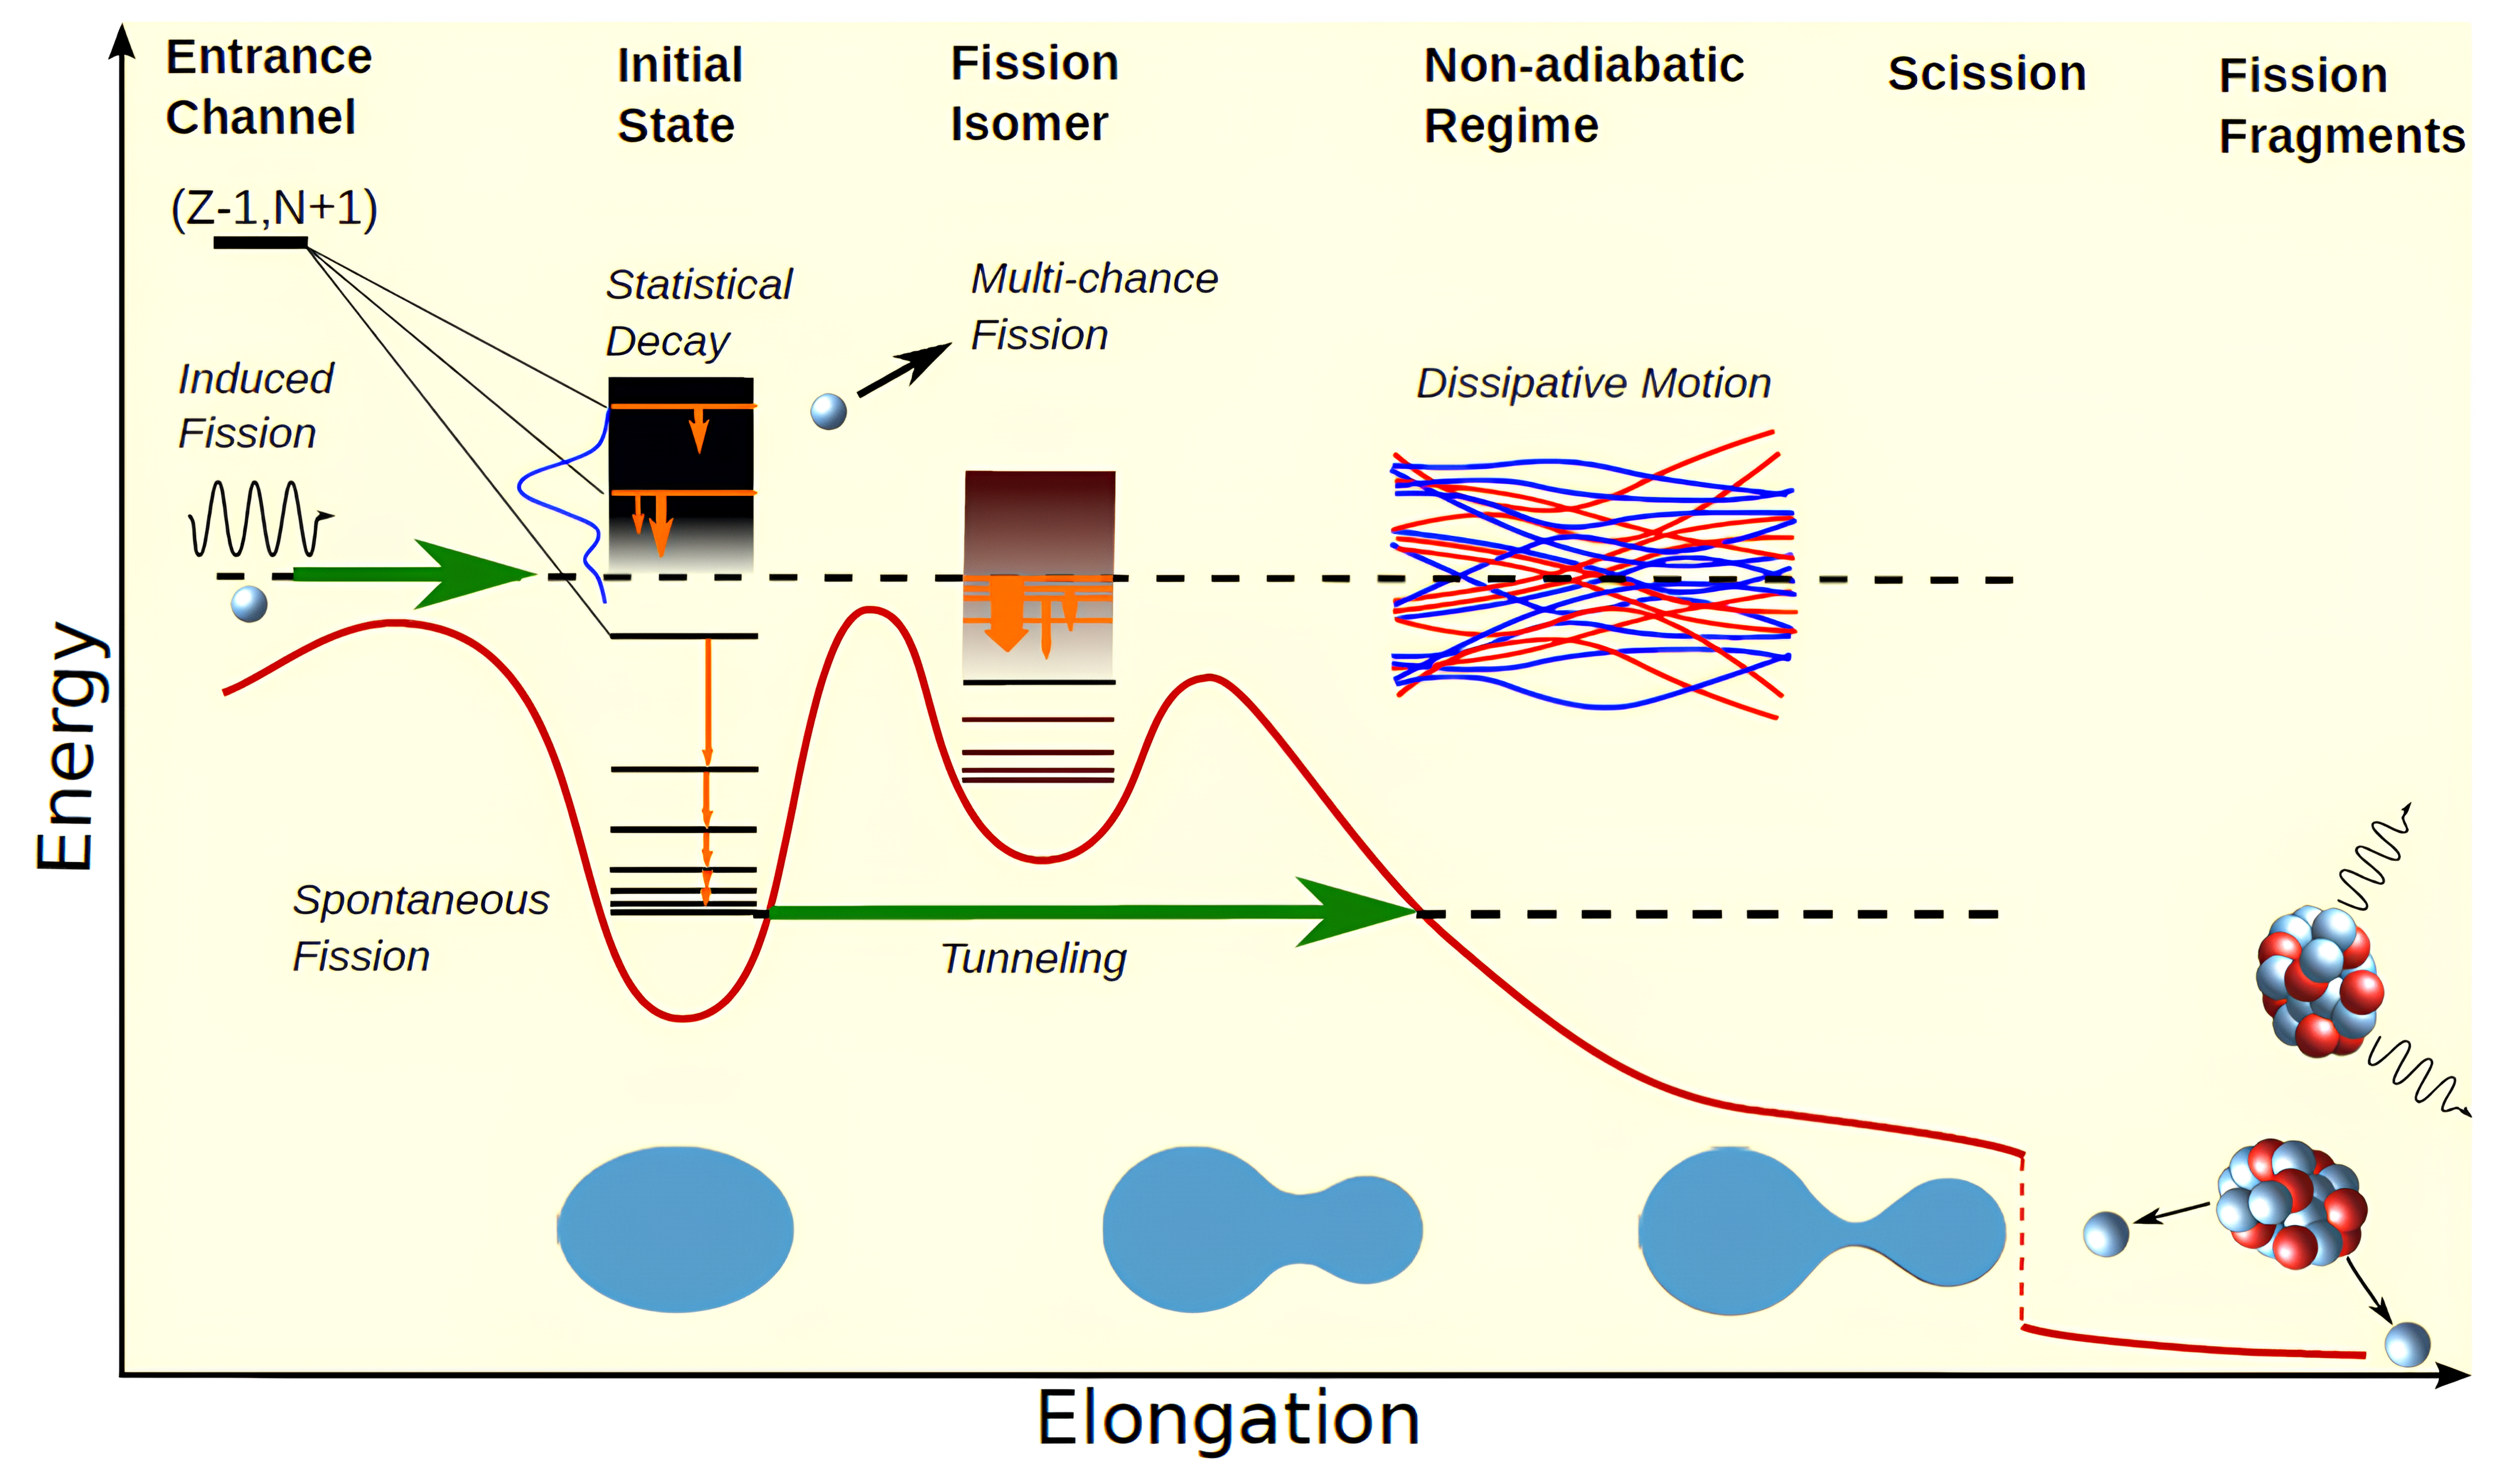
\includegraphics[width=0.85\textwidth]{Images/fission.png}
    \caption{Visual representation of the fission process. Figure taken from \cite{Bender2020}.}
    \label{fig:fission}
\end{figure}

\subsubsection{Spontaneous fission model}
It should be ovious that a formal treatment of deformations and collective modes is necessary to give a theoretical description of fission reactions. We can derive a simple spontaneous fission model by studying the effect of an axial quadrupole deformation on the semiempirical mass formula \ref{eq:semf}.

Let us assume that the nuclear radius may be expanded, as previously done in section \ref{sec:deformations}, as
\begin{equation}
    R = R_0[1+\alpha_{20}Y_{20}].
\end{equation}
Assuming the nuclear volume is conserved across the fission path, the volume energy will not change. As for the surface energy, its variation can be expressed at the lowest order in $\alpha_{20}$ as
\begin{equation}
    \Delta E_\text{surf} = E_\text{surf}
    -E_{0,\text{surf}} = E_{0, \text{surf}}\frac 2 5 \alpha_{20}^2.
\end{equation}
Regarding the Coulomb energy, the variation is given by
\begin{equation}
    \Delta E_\text{coul} = E_\text{coul} - E_{0, \text{coul}} = -E_{0, \text{coul}}\frac 1 5 \alpha_{20}.
\end{equation}
Since the neutron and proton numbers does not change, the surface and Coulomb energies are the only contributions to the total energy difference. We can write
\begin{equation}
    \label{eq:fission_semf}
    \Delta E = \frac 2 5 \alpha_{20}^2 a_s A^{2/3}- \frac 1 5 \alpha_{20}^2 a_c Z^2 A^{-1/3},
\end{equation}
if we set equation \eqref{eq:fission_semf} to zero, we get, other than the undeformed solution for $\alpha_{20}=0$, 
\begin{equation}
    \frac{ Z^2}{A} = \frac{2 a_s}{a_c},
\end{equation}
where the ratio $2a_s/a_c$ amounts to $\approx 50$ in typical parametrizations of the SEMF. Equation \eqref{eq:fission_semf}, shows that for values of the so called \textit{fissility parameter} $Z^2/A$ larger than $50$, the energy change becomes negative, favouring a configuration in which the nucleus fragments due to the spontaneous fission.
\subsection{Symmetry breaking and microscopic approaches to fission}
\subsubsection{Microscopic theory}
The use of phenomenological macroscopic-microscopic models has long provided valuable insight into fission processes, allowing for the prediction of barrier heights and fragment yields through parametrised shape degrees of freedom and empirical shell corrections \cite{Brack1972,Bjornholm1980,Krappe2012}.  
In these models, the total energy is expressed as
\begin{equation}
E_{\mathrm{tot}}(\boldsymbol{q}) = E_{\mathrm{LD}}(\boldsymbol{q}) + \delta E_{\mathrm{shell}}(\boldsymbol{q}) + \delta E_{\mathrm{pair}}(\boldsymbol{q}),
\end{equation}
where $E_{\mathrm{LD}}$ is the macroscopic liquid-drop term depending on deformation coordinates $\boldsymbol{q}$, while $\delta E_{\mathrm{shell}}$ and $\delta E_{\mathrm{pair}}$ account for shell and pairing corrections, respectively.  
While such models reproduce many global observables, they lack a true microscopic foundation.  
In particular, the collective coordinates $\boldsymbol{q}$ are not derived from the underlying many-body dynamics, and the empirical shell corrections cannot describe the self-consistent rearrangement of the mean field along the fission path.

A more fundamental understanding is achieved within self-consistent mean-field approaches such as the Hartree-Fock or Hartree-Fock-Bogoliubov formalisms. The use of nuclear Density Functional Theory \cite{Bender2003,Schunck2016} allows one to define a universal EDF $E[\rho,\kappa]$ that encapsulates both mean-field and pairing correlations.  
The resulting constrained HF/HFB calculations produce the potential energy surface (PES) $E(\boldsymbol{q})$, mapping the energy of the system as a function of collective deformations such as the quadrupole ($Q_{20}$), octupole ($Q_{30}$), and triaxial ($Q_{22}$) moments.  
The minima and saddle points of this multidimensional PES determine the fission barriers and shape isomeric states \cite{Dubray2012,Schunck2016}.

However, static mean-field approaches are limited by their single-reference character: the HFB vacuum represents only one configuration at a time, typically corresponding to a local minimum of the PES.  
In the vicinity of the fission barrier, where several configurations with different intrinsic quantum numbers coexist, this approximation breaks down.  
The wave function should instead be expressed as a superposition of several self-consistent configurations $\{|\Phi(\boldsymbol{q})\rangle\}$, leading to a correlated state of the form
\begin{equation}
|\Psi\rangle = \int f(\boldsymbol{q})\, |\Phi(\boldsymbol{q})\rangle\, d\boldsymbol{q},
\end{equation}
which is the essence of the \emph{Generator Coordinate Method} (GCM) \cite{Goutte2005,Regnier2019}.  
The GCM maps the microscopic many-body problem onto a \emph{collective Schrödinger equation} (CSE)
\begin{equation}
\left[ -\frac{\hbar^2}{2}\sum_{ij}\frac{\partial}{\partial q_i} B_{ij}(\boldsymbol{q}) \frac{\partial}{\partial q_j} + V(\boldsymbol{q}) \right] g_k(\boldsymbol{q})
= E_k g_k(\boldsymbol{q}),
\end{equation}
where $B_{ij}(\boldsymbol{q})$ is the collective inertia tensor and $V(\boldsymbol{q})$ the potential energy extracted from constrained HFB.  
This framework naturally incorporates tunnelling through the barrier and provides access to observables such as fission lifetimes and fragment distributions.  

Beyond-mean-field extensions also restore symmetries that are spontaneously broken at the mean-field level.  
For instance, particle-number, parity, and angular-momentum projection techniques \cite{Bender2004,Samyn2005} are required to recover good quantum numbers and remove spurious symmetry mixing.  
In multi-reference DFT \cite{Bender2003}, these symmetry restorations can be combined with configuration mixing, yielding highly accurate fission barrier calculations.  

\subsubsection{Unconstrained Calculations and Symmetry Breaking}

An equally important aspect of microscopic fission theory is the treatment of spatial symmetries.  
Historically, many calculations imposed constraints such as axial symmetry or reflection symmetry with respect to a plane to reduce the computational cost of solving the HFB equations.  
While such restrictions simplify the description of the nucleus, they artificially constrain the fission path and may even prevent the identification of energetically preferred configurations \cite{Warda2002,Bertsch2018}, as shown in figure \ref{fig:fission_barrier}.  
Fission involves strongly deformed, triaxial, and reflection-asymmetric shapes; the correct description of barrier heights and scission configurations therefore requires breaking as many spatial symmetries as possible.

In the self-consistent mean-field framework, spontaneous symmetry breaking is a feature rather than a flaw: it allows the system to adopt a deformed intrinsic shape corresponding to a broken rotational or parity symmetry, while the symmetry of the total many-body Hamiltonian is preserved.  
For example, an axially deformed HFB state violates rotational invariance, but the restoration of this symmetry through angular-momentum projection recovers the correct laboratory-frame properties.  
Similarly, parity breaking through octupole deformation is essential to describe asymmetric fission fragment distributions. Triaxiality, for example, has been shown to lower the inner barrier of actinides by several MeV \cite{Warda2002,Schunck2016}.
Likewise, reflection-asymmetric (octupole) degrees of freedom are necessary to reproduce mass-asymmetric fission in heavy nuclei.

Recent computational developments have made possible fully symmetry-unrestricted HFB and TDDFT calculations, in which all spatial and time-reversal symmetries can be broken if energetically favourable \cite{Simenel2018,Schunck2016}.  
Codes such as \texttt{HFODD} and \texttt{Sky3D} implement three-dimensional solvers capable of describing triaxial, octupole, and time-odd components of the density matrix.  
These advances have revealed new fission pathways, scission configurations, and fragment-spin correlations inaccessible to axially symmetric models.

In summary, microscopic theories based on DFT and its extensions offer a self-consistent foundation for the description of nuclear fission.  
They provide direct access to the interplay between shell effects, pairing, and deformation, which determine the shape evolution from the ground state to scission.  
